
\documentclass[submit]{harvardml}

% Put in your full name and email address.
\name{Your Name}
\email{email@fas.harvard.edu}

% List any people you worked with.
\collaborators{%
  John Doe,
  Fred Doe
}

% You don't need to change these.
\course{CS181-S18}
\assignment{Assignment \#4}
\duedate{11:59pm March 30, 2018} % FDV: Update due date 

\usepackage[OT1]{fontenc}
\usepackage[colorlinks,citecolor=blue,urlcolor=blue]{hyperref}
\usepackage[pdftex]{graphicx}
\usepackage{subfig}
\usepackage{fullpage}
\usepackage{amsmath}
\usepackage{amssymb}
\usepackage{color}
\usepackage{todonotes}
\usepackage{listings}
\usepackage{common}
\usepackage{bm}

\usepackage[mmddyyyy,hhmmss]{datetime}

\definecolor{verbgray}{gray}{0.9}

\lstnewenvironment{csv}{%
  \lstset{backgroundcolor=\color{verbgray},
  frame=single,
  framerule=0pt,
  basicstyle=\ttfamily,
  columns=fullflexible}}{}

\begin{document}
\begin{center}
{\Large Homework 4: Clustering and EM}\\
\end{center}


This homework assignment focuses on different unsupervised learning
methods from a theoretical and practical standpoint.  In Problem 1,
you will explore Hierarchical Clustering and experiment with how the
choice of distance metrics can alter the behavior of the algorithm. In
Problem 2, you will derive from scratch the full
expectation-maximization algorithm for fitting a Gaussian mixture
model. In Problem 3, you will implement K-Means clustering on a
dataset of handwritten images and analyze the latent structure learned
by this algorithm.

There is a mathematical component and a programming component to this
homework.  Please submit your PDF and Python files to Canvas, and push
all of your work to your GitHub repository. If a question requires you
to make any plots, please include those in the writeup.



\newpage
\section*{Hierarchical Clustering [7 pts]}

At each step of hierarchical clustering, the two most similar clusters
are merged together. This step is repeated until there is one single
group. We saw in class that hierarchical clustering will return a
different result based on the pointwise-distance and cluster-distance
that is is used. In this problem you will examine different choices of
pointwise distance (specified through choice of norm) and cluster
distance, and explore how these choices change how the HAC algorithm
runs on a toy data set.


\vspace{0.25cm}

\begin{problem}
~

 Consider the following four data points in $\reals^2$, belonging to three clusters: the
  black cluster consisting of $\boldx_1 = (0.1, 0.5) $ and $\boldx_2 = (0.35, 0.75))$,
  the red cluster consisting of $\boldx_3 = (0.28, 1.35)$, and the blue cluster
  consisting of $\boldx_4 = (0, 1.01)$.

  \begin{center} 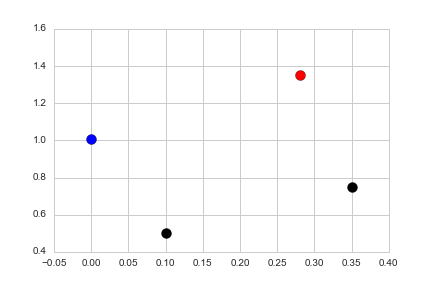
\includegraphics[scale=.3]{scatterplot.png} \end{center}


  Different pointwise distances $d(\boldx, \boldx') = \|\boldx - \boldx'\|_p$
  can be used.  Recall the definition of the
  $\ell_1$, $\ell_2$, and $\ell_{\infty}$ norm:
  \begin{eqnarray*}
     \| \mathbf{x} \|_1 = \sum_{j = 1}^m |x_i| \quad \quad\quad \| \mathbf{x} \|_2 = \sqrt{\sum_{j = 1}^m x_i^2 } \quad\quad\quad
     \| \mathbf{x} \|_{\infty} = \max_{j \in \{1, \ldots, m\}} |x_j|\\
  \end{eqnarray*}
  
  Also recall the definition of min-distance, max-distance,
  centroid-distance, and average-distance between two clusters (where $\bmu_{G}$
is the center of a cluster $G$):
%
\begin{eqnarray*}
    d_{\text{min}}(G, G') &=& \min_{\boldx  \in G, \boldx' \in G'} d(\boldx, \boldx')\\
    d_{\text{max}}(G, G') &=& \max_{\boldx  \in G, \boldx' \in G'} d(\boldx, \boldx')\\
    d_{\text{centroid}}(G, G') &=&  d(\bmu_{G}, \bmu_{G'})\\
    d_{\text{avg}}(G, G') &=&\frac{1}{|G| |G'|} \sum_{\boldx \in G}\sum_{\boldx'  \in G'} d(\boldx, \boldx')\\
  \end{eqnarray*}

  \begin{enumerate}
  \item Draw the 2D unit sphere for each norm,
  defined as $\mathcal{S} = \{\boldx \in \mathbb{R}^2: \|\boldx\| = 1 \}$. Feel free to do
  it by hand, take a picture and include it in your pdf.
\item  For each norm ($\ell_1, \ell_2, \ell_\infty$) and each clustering distance, specify which two clusters would
  be the first to merge.
\item Draw the complete dendrograms showing the order of agglomerations for the $\ell_2$ norm and each of the clustering distances. We have provided some code to make this easier for you. You are not required to use it.
  \end{enumerate}


\end{problem}

\subsection*{Solution}

\newpage 

\section*{Expectation-Maximization for Gaussian Mixture Models [7pts]}


In this problem we will explore expectation-maximization for the
Gaussian Mixture model.  Each observation $\boldx_i$ is a vector in
$\mathbb{R}^{D}$.  We posit that each observation comes from
\emph{one} mixture component.  For this problem, we will assume there
are $c$~components. Each component $k \in \{1, \ldots, c\}$ will be
associated with a mean vector $\mu_k \in R^{D}$ and a covariance
$\Sigma_k$.  Finally let the (unknown) overall mixing proportion of
the components be~$\btheta \in [0,1]^c$, where~${\sum_{k=1}^c
  \theta_k=1}$.

Our generative model is that each of the~$n$ observations comes from a
single component.  We encode observation $i$'s component-assignment as
a one-hot vector~${\boldz_i \in \{0,1\}^c}$ over components. This
one-hot vector is drawn from~$\btheta$; then, $\boldx_i$ is drawn
from~$N(\mu_{z_i}, \Sigma_{z_i})$. Formally documents are generated in two steps:
\begin{eqnarray*}
 \boldz_i &\sim& \text{Categorical}(\btheta) \\
 \boldx_i &\sim& N(\mu_{z_i}, \Sigma_{z_i})
\end{eqnarray*}


\begin{problem}
  ~

  \begin{enumerate}

    % FDV mostly at Mark Goldstein, delete once read: changed to be
    % intractability of the data likelihood because we don't have
    % priors over the mus and Sigmas in this problem.  We could change
    % the whole problem to add priors, but that might be too hard/a
    % better problem for 281... 
  \item \textbf{Intractability of the Data Likelihood} Let $\phi_k$
    represent all the parameters associated with a component
    $(\mu_k,\Sigma_k)$.  We are generally interested in finding a set
    of parameters $\phi_k$ that maximize the data likelihood $\log
    p(\{x_i\}|\{phi_k\})$.  Expand the data likelihood to include the
    necessary sums over observations $x_i$ and latents $z_i$.  Why is
    optimizing this loss directly intractable?
    
\item \textbf{Complete-Data Log Likelihood} Define the complete data for this problem to be $D = \{(\boldx_i, \boldz_i)\}_{i=1}^n$. Write out the complete-data (negative) log likelihood. \[\mcL(\btheta, \{\mu_k,\Sigma_k\}^c_{k=1}) =  -\ln p(D \given\btheta, \{\mu_k,\Sigma_k\}^c_{k=1}).\] 
    

\item \textbf{Expectation Step}
Our next step is to introduce a mathematical expression for $\boldq_i$, the posterior over the hidden topic variables~$\boldz_i$ conditioned on the observed data $\boldx_i$ with fixed parameters, i.e $p(\boldz_i | \boldx_i; \btheta, \{ \mu_k,\Sigma_k \}^c_{k=1})$.

\begin{itemize}
\item  Write down and simplify the expression for $\boldq_i$. 
\item  Give an algorithm for calculating $\boldq_i$ for all $i$, given the observed data~$\{\boldx_i\}^n_{i=1}$ and settings of the parameters~$\btheta$ and~$\{ \mu_k,\Sigma_k  \}^c_{k=1}$.

\end{itemize}

\item \textbf{Maximization Step}
Using the~$\boldq_i$ estimates from the Expectation Step, derive an update for maximizing the expected complete data log likelihood in terms of~$\btheta$ and~$\{ \mu_k,\Sigma_k \}^c_{k=1}$.

\begin{itemize}
    \item Derive an expression for the expected complete-data log likelihood in terms of $\boldq_i$.
    \item Find an expression for $\btheta$ that maximizes this expected complete-data log likelihood. You may find it helpful to use Lagrange multipliers in order to force the constraint $\sum \theta_k = 1$. Why does this optimized $\btheta$ make intuitive sense?
    \item Apply a similar argument to find the value of the $(\mu_k,\Sigma_k)$'s that maximizes the expected complete-data log likelihood. 
\end{itemize}

\item Finally, compare this EM approach to the generative model for
classification in Homework 2.  How are the computations similar?
Different? 

\end{enumerate}


  
\end{problem}

\subsection*{Solution}


\newpage

\section*{K-Means [15 pts]} % FDV: Any more interesting data sets?  

For this problem you will implement  K-Means clustering from scratch. Using \texttt{numpy} is fine, but don't use a
third-party machine learning implementation like \texttt{scikit-learn}. You will then apply this approach to clustering of image data.  



We have provided you with the MNIST dataset, a collection of handwritten digits used as a benchmark of image recogntion (you  can
learn more about the data set at  \url{http://yann.lecun.com/exdb/mnist/}). The MNIST task
is widely used in supervised learning, and modern algorithms with neural
networks do very well on this task. 

Here we will use MNIST unsupervised learning. You have been given
representations of 6000 MNIST images, each of which are $28\times28$
greyscale handwritten digits. Your job is to implement K-means
clustering on MNIST, and to test whether this relatively simple algorithm can
cluster similar-looking images together.

~

\begin{problem}
The given code loads the images into your environment as a 6000x28x28 array.

\begin{itemize}
\item Implement K-means clustering
from different random initializations 
and for several values of $K$ using the 
$\ell_2$ norm as your
distance metric. (You should feel free to explore other metrics 
than the $\ell_2$ norm, but this is strictly optional.)  Compare the 
K-means objective for different values of K and across random
initializations.
%
\item For three different values of K,
and a couple of random restarts for each, 
show the mean images for each cluster (i.e., for
the cluster prototypes), as well as the images for a 
few representative images for each cluster. You should explain how you selected
these representative images. To render an image, use the pyplot \texttt{imshow} function. 

\item Are the results wildly different for different
restarts and/or different 
values of K?
For one of your runs, plot the K-means objective function as a function of iteration and verify that
it never increases.

%\item Finally, implement K-means++ and see if gives you more satisfying
%initializations (and final results) for K-means. Explain your findings.

\end{itemize}


As in past problem sets, please include your plots in this
document. (There may be several plots for this problem, so feel free
to take up multiple pages.)




\end{problem}
\subsection*{Solution}


%Figure out how to load it into your environment and turn it into a set of
%vectors.  Run K-Means on it for a few different~$K$ and show some results from
%the fit.  What do the mean images look like?  What are some representative
%images from each of the clusters?  Are the results wildly different for
%different restarts and/or different~$K$?  Plot the K-Means objective function
%(distortion measure) as a function of iteration and verify that it never
%increases.

%\subsection*{4. Implement K-Means++ [4 pts]} mplement K-Means++ and see if it
%gives you more satisfying initializations for K-Means.  Explain your findings.

\newpage
\begin{problem}[Calibration, 1pt]
Approximately how long did this homework take you to complete?
\end{problem}


\end{document}
